\documentclass[a4paper]{scrreprt}

\usepackage[german]{babel}
\usepackage[utf8]{inputenc}
\usepackage[T1]{fontenc}
\usepackage{ae}
\usepackage{amssymb}
\usepackage{graphicx}
\usepackage{hyperref}

\begin{document}

m\title{BS Zusammenfassung}
\author{Benedict Hauck, Fedor Scholz}
\maketitle

\tableofcontents
\vspace{1cm}

\chapter{01aIntro}

\section{Was ist ein Betriebssystem?}

\begin{itemize}
	\item Vermittler zwischen Benutzer und Computer
	\item Ziele
		\begin{itemize}
			\item Benutzerprogramme ausfuehren und dem Benutzer das Loesen von Problemen erleichtern
			\item Computer benutzbarer machen
			\item Hardware des Computer effizient nutzen
		\end{itemize}
	\item Vier Komponenten eines Computersystems
		\begin{itemize}
			\item Benutzer
			\item System- und Anwendungsprogramme
			\item Betriebssystem
			\item Hardware
		\end{itemize}
	\item Betriebssysteme verteilen Ressourcen
		\begin{itemize}
			\item Verwaltung aller Ressourcen
			\item Entscheidung bei konfligierenden Anfragen fuer effizientes und faires Benutzen der Ressourcen
		\end{itemize}
	\item Betriebssysteme kontrollieren
		\begin{itemize}
			\item Kontrolle von Ausfuehrungen von Programmen um Fehler und ungeeignetes Benutzen des Computers zu verhindern
		\end{itemize}
	\item Das Programm, welches immer laeuft, ist der Kernel. Alles andere ist entweder ein System- oder Anwendungsprogramm
	\item Das bootstrap program wird beim Starten oder Neustarten geladen
		\begin{itemize}
			\item Wird in ROM, EPROM oder FLASH als firmware gespeichert
			\item Initialisiert alle Aspekte des Systems, insbesondere die HW-Komponenten
			\item Laedt den Kernel und startet die Ausfuehrung
		\end{itemize}
\end{itemize}

\section{Organisation}

\begin{itemize}
	\item Ein oder mehr CPUs, device controllers verbinden sich ueber den Bus um Zugriff auf shared memory zu bekommen
	\item I/O-Geraete und CPU koennen gleichzeitig ausfuehren
	\item Jeder device controller ist zustaendig fuer einen Geraetetypen
	\item Jeder device controller hat einen lokalen Puffer
	\item CPU bewegt Daten vom/zum Hauptspeicher zu/von lokalen Puffern
	\item I/O ist vom Geraet zum lokalen Puffer des controllers
	\item device controller informiert CPU per interrupts, wenn er fertig ist
\end{itemize}


\section{Interrupts}

\subsection{Haeufige Funktionen von Interrupts}

\begin{itemize}
	\item interrupt gibt Kontrolle an interrupt service routine ueber einen interrupt vector, welcher die Adressen von allen service routines beinhaltet
	\item interrupt architecture muss Adresse der unterbrochenen Intruktion speichern
	\item Einkommende interrupts sind aus, wenn gerade ein anderer bearbeitet wird um lost interrupts zu verhindern
	\item trap ist ein interrupt, welcher von Software verursacht wurde (wegen eines Fehler oder durch eine Benutzeranfrage)
	\item Betriebssysteme sind interrupt driven
\end{itemize}

\subsection{Timer interrupts}

\begin{itemize}
	\item Time interrupts um endlose Schleifen und Prozesse zu verhindern
	\item Wird nach bestimmter Zeitspanne ausgefuehrt
	\item Wird vor dem schedulen des Programm aufgesetzt
	\item Eingebettete Systeme haben Watchdog, welche bis 0 zaehlt und dann resettet
\end{itemize}

\subsection{Interrupt Handling}

\begin{itemize}
	\item Betriebssystem merkt sich Status der CPU, indem es Register und Programmzaehler speichert
	\item Legt Typ des interrupts fest
		\begin{itemize}
			\item polling
			\item vectored interrupt system
		\end{itemize}
\end{itemize}

\section{I/O Struktur}

\subsection{Synchrone oder blockende I/O}

\begin{itemize}
	\item Nachdem I/O beginnt, geht die Kontrolle erst nach Fertigstellung der I/O wieder zum Benutzerprogramm
	\item Wait instruction laesst die CPU idlen
	\item Meistens nur ein I/O Request gleichzeitig
	\item Polling
	\item Signal
	\item Callback function
\end{itemize}

\subsection{Direct Memory Access Structure}

\begin{itemize}
	\item Fuer high-speed I/O, damit diese mit fast der Geschwindigkeit des Hauptspeichers Informationen uebertragen koennen
	\item Device Controller uebertraegt Daten in Bloecken vom Puffer direkt in den Hauptspeicher ohne CPU Eingriff
	\item Nur ein interrupt pro Block
\end{itemize}

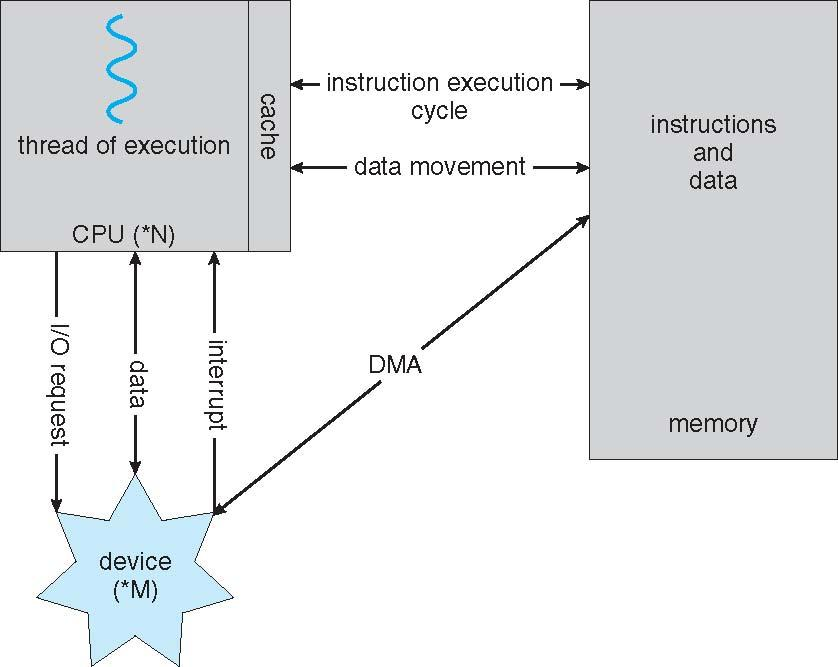
\includegraphics[scale=0.4]{dma.png}









\chapter{01bCProgramming}
\chapter{02OS}

\section{Monolithisches System}
Vorteile:
	\begin{itemize} 
		\item Einfacher Zugriff auf alle Systemdaten 
		\item Kosten von Modulinteraktionen sind niedrig
		\item Erweiterbar über Schnittstellen
		\item Vorhersehbares Verhalten 
	\end{itemize}
Nachteile:
	\begin{itemize}
		\item Kein Schutz zwischen System und Anwendung
		\item Instabil
	\end{itemize}

Beispiele:
	\begin{itemize}
		\item uCLinux, RTOSe, eCos
	\end{itemize}
	
\section{Mehrschichtiger Ansatz}
	\begin{itemize}
		\item Betriebssystem ist in n Schichten aufgeteilt
		\item Jede Schicht kann nur auf die Funktionen und Dienste von niedrigeren Schichten zugreifen 
			\begin{itemize} 
				\item Schicht 0 ist die Hardware
				\item Schicht n ist das Benutzerinterface
			\end{itemize}
		\item Einfachere Migration zwischen Plattformen
		\item Einfachere Evolution der Hardwareplattform
		\item Niedrigere Schichten implementieren Mechanismen
		\item Höhere Schichten implementieren meistens Policies
	\end{itemize}

\begin{center}
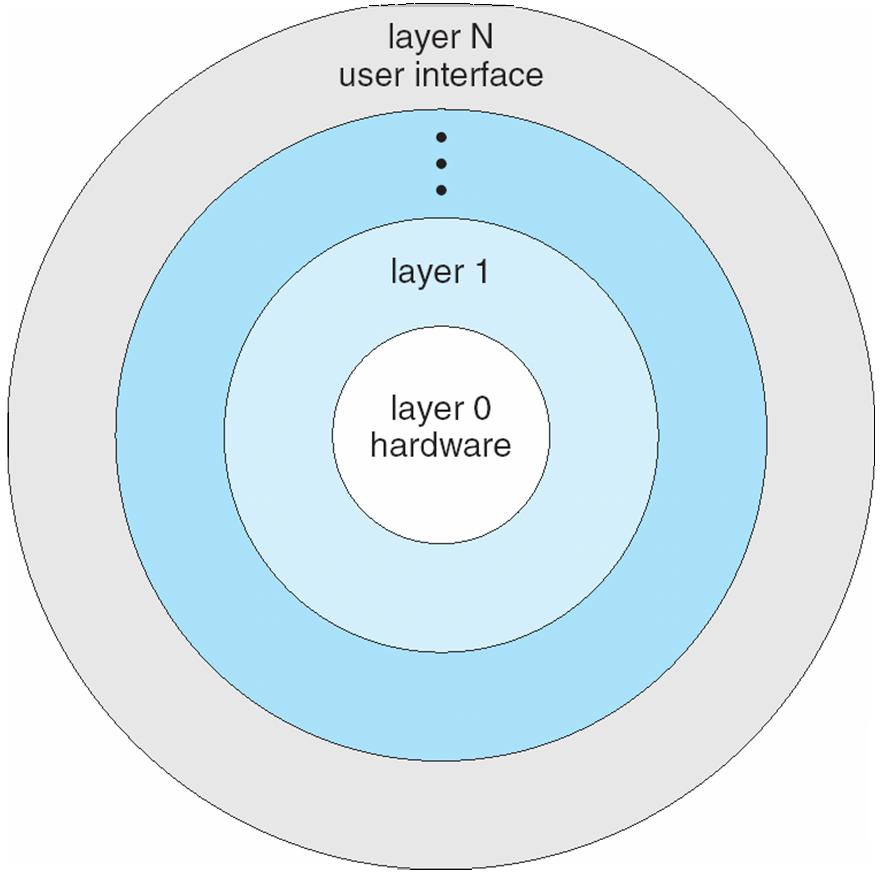
\includegraphics[scale=0.15] {schichtenmodell.png} 
\end{center}

Vorteile:
	\begin{itemize}
		\item Jede Schicht kann unabhängig getestet und verfiziert werden
		\item Korrektheit von Schicht n hängt nur von Schicht n-1 ab (einfacheres Debugging, einfachere Wartung)
	\end{itemize}

Nachteile:
	\begin{itemize}
		\item Nur unidirektionaler Schutz
		\item Beiseitige Abhängigkeit von Schichten verhindert strikte Schichtenbildung
	\end{itemize}
Beispiele:
	\begin{itemize}
		\item THE (Dijkstra), Multics(GE), VOCOS(EWSD)
	\end{itemize}
	
\section{Monolitische Kernels}
	\begin{center}
		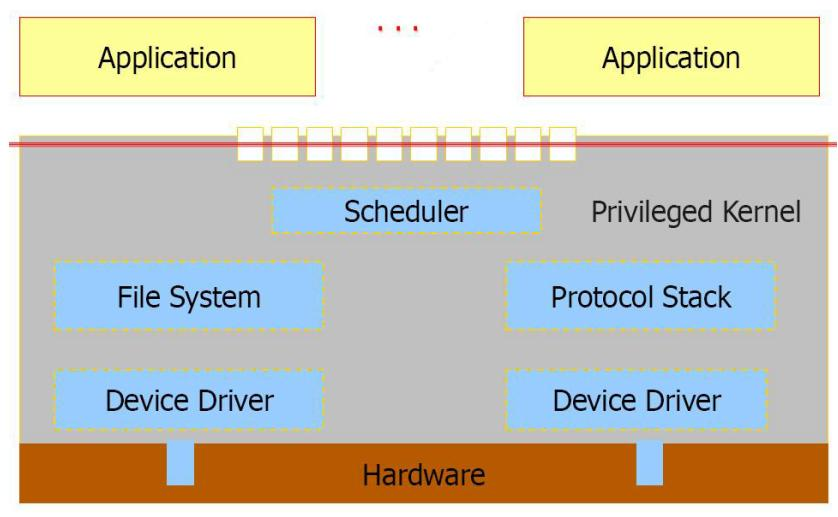
\includegraphics[scale=0.3] {monolithickernel.png}
	\end{center}
	Vorteile:
		\begin{itemize}
			\item "Gute" Performance
			\item Ausreichender Schutz zwischen Anwendungen
			\item Erweiterbar über Schnittstellen und statische/ladbare Module
		\end{itemize}
	Nachteile:
		\begin{itemize}
			\item Kein Schutz zwischen Kernel-Komponenten
			\item Nebeneffekte durch undokumentierte Interfaces
			\item Hohe Komplexität durch hohe gegenseitige Abhängigkeit
		\end{itemize}
	Beispiele
		\begin{itemize}
			\item Linux, Solaris
		\end{itemize}

\section{Microkernel Systeme}
	\begin{center}
		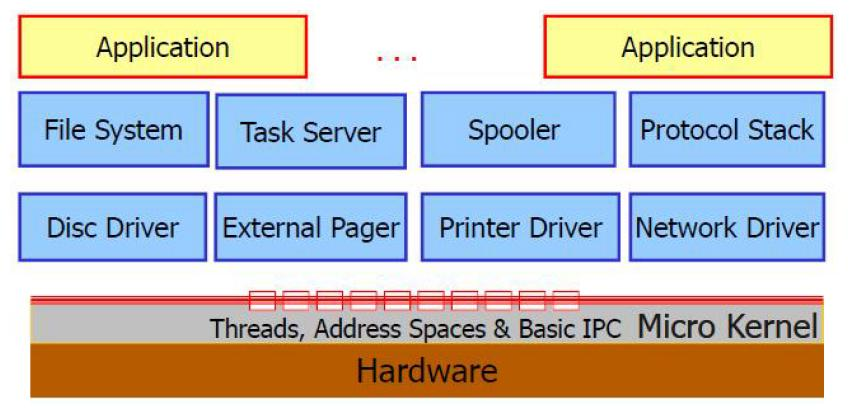
\includegraphics[scale=0.3] {microkernel.png}
	\end{center}

	\begin{itemize}
		\item Möglichst viel des Kernels in den "Benutzer" space packen
		\item Kommunikation erfolgt zwischen Benutzermodulen mit Nachrichtenweitergabe
	\end{itemize}
	
	Vorteile:
		\begin{itemize}
			\item Einfacher einen Microkernel zu erweitern
			\item Einfacher das Betriebssystem auf neue Architekturen zu portieren
			\item Zuverlässiger (es läuft weniger Code im Kernel-Modul
			\item Mehrere APIs vorhanden
			\item Verbesserte Robustheit und Sicherheit
			\item Einfacher zum Testen und Beweisen
			\item Verbesserte Wartbarkeit
		\end{itemize}
	Nachteile:
		\begin{itemize}
			\item Performance Unkosten durch Kommunikation von Benutzerspace zum Kernelspace 
			\item Zusätzliche Zersetzung
			\item Schlechte Erfahrungen mit IBMs Workplace OS (1991-1995)
		\end{itemize}

\section{Virtuelle Maschinen}
	\begin{itemize}
		\item Eine virtuelle Maschine nimmt den mehrschichtigen Ansatz und behandelt Hardware sowie den Kernel des Betriebssystems so als wären sie Hardware
		\item Eine virtuelle Maschine stellt ein identisches Interface zu der blanken, darunterliegenden Hardware
		\item Der Betriebssystem-Host kreiert die Illusion das ein Prozess sein eigenen Prozessor und (virtuellen Speicher) hat.
		\item Jeder Gast bekommt eine Kopie des darunterliegenden Computers zur Verfügung gestellt.
	\end{itemize}
	Vorteile:
		\begin{itemize}
			\item Mehrere Betriebssysteme können sich die gleiche Hardware teilen
			\item Gegenseitiger Schutz
			\item Nützlich für Development und Testen
		\end{itemize}
	\begin{center}
		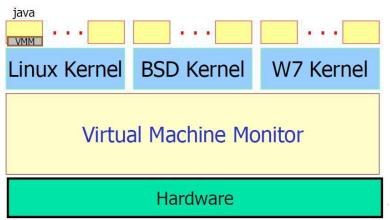
\includegraphics[scale=0.5] {virtualmachine.png}
		\\
		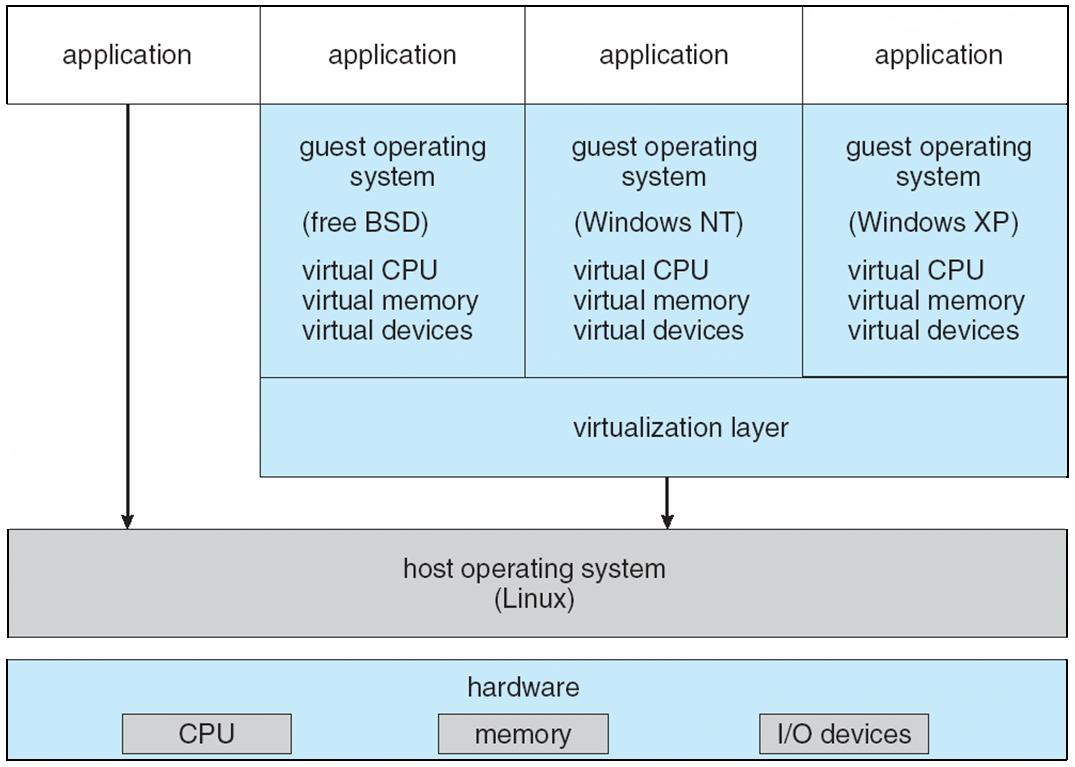
\includegraphics[scale=0.35] {vmwarearchi.png}
		\\
		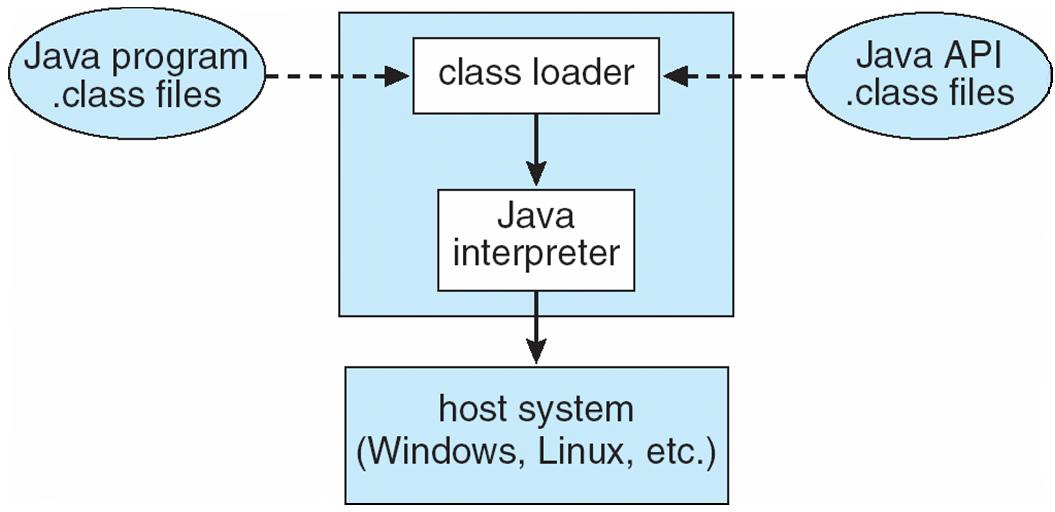
\includegraphics[scale=0.3] {javavm.png}
	\end{center}


\chapter{03aProcess-management}
\chapter{03bProcess-management-scheduling}
\chapter{04Process-coordination}

\section{Interprozess Kommunikation}
	\begin{itemize}
		\item Prozesse in einem System können unabhängig oder zusammenarbeitend sein
		\item Zusammenarbeitende Prozesse können sich andere oder von anderen Prozessen beeinflusst werden
		\item Zusammenarbeitende Prozesse benötigen interprocess communication (IPC -> 2 Modelle: Shared memory, message passing)
	\end{itemize}
	Gründe für zusammenarbeitende Prozesse:
	\begin{itemize}
		\item Schnellere Berechnung
		\item Kompfort/Einfachheit
		\item Modularität
		\item Teilen von Informationen
	\end{itemize}

\subsection{Nachrichtenweitergabe (Message Passing)}
	\begin{itemize}
		\item Mechanismus für Prozesse um zu kommunizieren und ihre Aktionen zu synchronisieren
		\item IPC-Einrichtung bietet zwei Operationen: receive, send (Nachrichtengröße ist fix oder variabel)
	\end{itemize}
\subsubsection {Direkte Kommunikation}
	\begin{itemize}
		\item Prozesse müssen sich gegenseitig explizit per Namen nennen
		\item send(P, Nachricht) - schicke eine Nachricht an Prozess P
	\end{itemize}
	Eigenschaften:
	\begin{itemize}
		\item Links werden automatisch eingerichtet
		\item Ein Link wird genau mit einem Paar von kommunizierenden Prozessen assoziiert
		\item Jedes Paar besitzt genau einen Link
		\item Ein Link könnte unidirektional sein, ist aber meistens bi-direktional
	\end{itemize}
	
\subsubsection{Indirekte Kommunikation}
	\begin{itemize}
		\item Nachrichten werden von Mailboxes (ports) gelenkt und empfangen
		\item Jede Mailbox hat eine einzigartige ID
		\item Prozesse können nur kommunizieren wenn sie eine Mailbox teilen
	\end{itemize}
	Eigenschaften:
	\begin{itemize}
		\item Ein Link wird nur eingerichtet falls Prozssse eine Mailbox teilen
		\item Ein Link kann mit vielen Prozessen assoziiert werden
		\item Jedes Paar von Prozessen kann mehere Kommunikationslinks teilen
		\item Links können unidirektional oder bi-direktional sein
	\end{itemize}
	Operationen:
	\begin{itemize}
		\item Neue Mailbox erstellen
		\item schicken und empfangen von Nachrichten über die Mailbox
		\item Mailbox löschen
	\end{itemize}
	
\section{Synchronisation}
	\subsection {Producer-Consumer Problem}
		\begin{itemize}
			\item Problemstellung der Prozesssynchronisation die eine Regelung der Zugriffsreihenfolge auf einer Datenstruktur von Prozessen bzw Thread thematisiert
			\item Prozesse sind Erzeuger oder Verbraucher
		\end{itemize}	
	\subsubsection{Critical-Section-Problem}
		\begin{itemize}
			\item Mutual Exclusion: Wenn Prozess P in seinem kritischen Bereich ist, kann kein anderer Prozess in seinen kritischen Bereich
			\item Progress:  Wenn kein Prozess in seinem kritischen Bereich ausgeführt wird, aber mehrere Prozesse den kritischen Bereich betreten möchten, kann die Auswahl der Prozesse die als nächstes eintreten nicht unbegrenzt aufgeschoben werden
			\item Bounded Waiting: Es muss eine zeitliche Grenze existieren, sodass Prozesse nicht verhungern. (z.B. Prozess A,B wechseln sich in im kritischen Bereich ab obwohl Prozess C auch den kritischen Bereich betreten möchte, Prozess C verhungert)
			\item Viele Systeme bieten Hardwaresupport für critical section code
		\end{itemize}
	\subsection{Semaphore}
		\begin{itemize}
			\item Synchronisationstool das kein "busy waiting" benötigt
			\item Weniger kompliziert
			\item Nur zwei Standardoperationen für die Modifikation eines Semaphores erlaubt: wait(), signal()
			\item Counting semaphore - integer Wert unbegrenzt
			\item Binary semaphore - integer Wert kann zwischen 0 und 1 variieren 
		\end{itemize}

\section{Deadlock and Starvation}
		\begin{itemize}
			\item Deadlock - zwei oder mehr Prozesse warten unbegrenzt auf eine Aktion die nur von einem wartenden Prozess ausgeführt werden kann
			\item Starvation - Ein Prozess könnte nie von einer Semaphorewarteschlange entfernt werden
			\item Priority Inversion - Scheduling-Problem, wenn ein Prozess niedriger Priorität einen Platz hält den ein Prozess höherer Priorität braucht
		\end{itemize}

\chapter{05aMemoryManagement}
\chapter{05bMemoryManagement}
\chapter{05cMemoryManagement}
\chapter{06aFileSystems}
\chapter{06bFileSystems}
\chapter{07aImplementingFileSystems}
\chapter{07bImplementingFileSystems}
\chapter{08SecondaryStorageStructure}
\chapter{09IoSystems}

\end{document}
